%%
%% ****** ljmsamp.tex 13.06.2018 ******
%%
\documentclass[
11pt,%
tightenlines,%
twoside,%
onecolumn,%
nofloats,%
nobibnotes,%
nofootinbib,%
superscriptaddress,%
noshowpacs,%
centertags]%
{revtex4}
\usepackage{ljm}
\usepackage{listings}

\lstset{
language=C,
basicstyle=\small\ttfamily,
numbers=left,
numberstyle=\tiny,
stepnumber=1,
numbersep=5pt,
showspaces=false,
showstringspaces=false,
showtabs=false,
frame=single,
tabsize=2,
captionpos=t,
breaklines=true,
breakatwhitespace=false,
escapeinside={\%*}{*)}
}

\begin{document}

\titlerunning{Vectorization with AVX-512 instructions} % for running heads
\authorrunning{A.~A.~Rybakov and S.~S.~Shumilin} % for running heads
%\authorrunning{First-Author, Second-Author} % for running heads

\title{Vectorization of High-performance Scientific Calculations\\
Using AVX-512 Intruction Set}
% Splitting into lines is performed by the command \\
% The title is written in accordance with the rules of capitalization.

\author{\firstname{A.~A.}~\surname{Rybakov}}
\email[E-mail: ]{rybakov.aax@gmail.com}
\affiliation{Joint Supercomputer Center of the Russian Academy of Sciences - branch of Scientific Research Institute of System Analysis of the Russian Academy of Sciences, Leninsky prospect 32a, Moscow, 119334, Russia}

\author{\firstname{S.~S.}~\surname{Shumilin}}
\email[E-mail: ]{shumilin@jscc.ru}
\affiliation{Joint Supercomputer Center of the Russian Academy of Sciences - branch of Scientific Research Institute of System Analysis of the Russian Academy of Sciences, Leninsky prospect 32a, Moscow, 119334, Russia}
%\noaffiliation % If the author does not specify a place of work.

\firstcollaboration{(Submitted by G.~I.~Savin)} % Add if you know submitter.
%\lastcollaboration{ }

\received{June 13, 2018} % The date of receipt to the editor, i.e. December 06, 2017


\begin{abstract} % You shouldn't use formulas and citations in the abstract.
abstract
\end{abstract}

\subclass{68N19} % Enter 2010 Mathematics Subject Classification.

\keywords{Optimization, vectorization, AVX-512, predicated execution, intrinsics, application performance.} % Include keywords separeted by comma.

\maketitle

% Text of article starts here.

\section{Introduction}

introduction

\section{Flat loops vectorization}

The simplest context for vectorization is a flat loop. We call a flat cycle with the following properties. First, it should not contain inter-iteration dependencies, that is, all loop iterations can be executed in parallel. Secondly, within the iteration of the loop with number i there can only be such memory access operations that read or write elements of arrays with indices i (all references to memory can be reduced to the form a [i]). A trivial example of a flat loop is the addition of two arrays. As a rule, flat loops containing only arithmetic operations are automatically compiled by the compiler and demonstrate multiple acceleration, since the AVX-512 instruction set contains vector analogues of all arithmetic operations. The situation is more complicated with vectorization of flat cycles containing singularities. As features may be, for example, conditional operators or control transfer commands. Such cycles are also easily vectorized, but in practice the compiler often refuses to build a vector code due to a theoretical estimate of the possible acceleration. The presence of a strongly branched control in a flat cycle usually leads to the rejection of vectorization, in such cases the vector code must be built manually. The more serious features that prevent the construction of an effective parallel code is the presence of nested loops or function calls in a flat loop. In this case, the compiler is not able to perform vectorization, although using the inrinsikov functions, optimization can also be performed in these cases.

Let us analyze in more detail the question of vectorization of flat cycles. Suppose that the vectorization uses vectors capable of containing w primitive data elements, in this case we will call w the vectorization width (AVX-512 vectors can contain 8 double elements or 16 float elements). We will not consider a variant in which the cycle body contains only arithmetic operations due to its triviality. Let the considered flat cycle contain n iterations. Then all iterations of this cycle can be divided into n / w groups by w iterations, and each group can be considered separately (a residual group of iterations containing less than w iterations is also possible; the presence of this group does not affect the optimization efficiency, it can be completed in the original form or vectorized using masks). Thus, for simplicity, we can restrict ourselves to the consideration of flat cycles containing exactly w iterations.

As a first example, we consider a planar cycle whose body consists of a single linear section of a block, which is executed under the condition cond with probability p and has a length t (see Fig. N, a). In this case, the length of a linear section is understood to be a characteristic proportional to the execution time of a given linear section (the number of operators, machine instructions or cycles). The total number of operations contained in the cycle is ptw (in this case, we assume that the auxiliary instructions related to the calculation of the condition and the provision of control can be neglected). If the probability that the condition cond is satisfied is low enough, then we can only stop at the vectorization of this condition and perform the whole cycle under this condition vcond. This transformation will be called the vectorization of the condition (see Fig. N, b). Moreover, the probability that the condition vcond turns out to be instinctive is $1 - (1 - p) ^ w$ (corresponds to the fact that at least one of the w elementary conditions is true). The total number of operations in the cycle from this conversion will not change (the cond and vcond conditions are not independent) and will remain equal to ptw, but the number of auxiliary operations and control operations will be reduced. To vectorize the entire cycle, it is necessary to convert the program code into a predicate code, in which each instruction of the linear section block is executed under the predicate cond, then all the instructions of the linear section can be replaced by vector analogs executed under the vector predicate vcond (see Fig. N, c ). The number of operations of a fully vectorized cycle is simply t. At the same time, it is also not forbidden to use vcond checking for voidness before executing vectorized code in order to avoid executing code blocks with empty masks (see Fig. N, d). In this case, the number of cycle operations will be reduced by $1 - (1 - p) ^ w$ times, since the addition of a condition will cut off the execution of vector operations with an empty mask.

\begin{figure}[h]
\setcaptionmargin{5mm}
%\onelinecaptionsfalse % if the caption is multiline
\onelinecaptionstrue  % if the caption is one-line
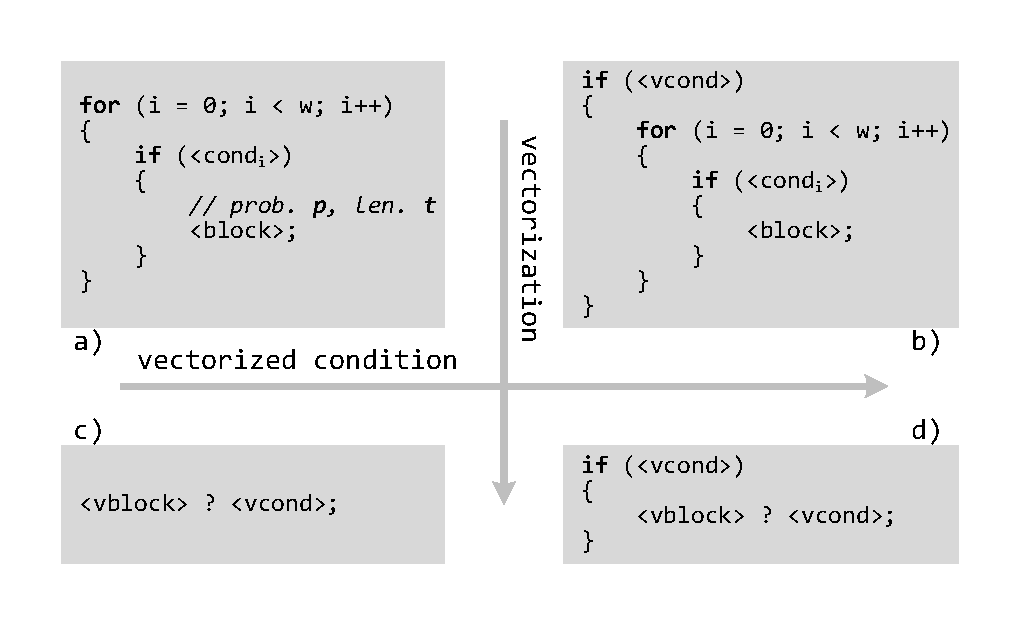
\includegraphics[width=0.62\textwidth]{pics/if_vectorization.pdf}
\captionstyle{normal}\caption{Please write your figure caption here.}\label{fig:1}
\end{figure}

As another example, consider a planar loop whose body is an if-else construct. Without loss of generality, we assume that the branch executed by the if-condition (block1) is more likely than its alternative (block2), that is, $p> = 1 - p$. The lengths of the linear sections in this example are t1 and t2, respectively (see Fig. N, a). In addition, we will assume that the block1 linear section is suitable for vectorization in any case, and a vector code is constructed for it (otherwise, the optimization of this code loses its meaning). The total number of operations performed during the cycle operation is calculated as the mathematical expectation of the number of operations per iteration multiplied by the number of iterations of the cycle, that is $(pt1 + (1 - p) t2) w$. In real computational problems, it often happens that an unlikely branch in such cycles does not lend itself to vectorization or this requires considerable effort. Such unlikely branches contain processing of extremely rare exceptions or unexpected situations. In such cases, it is natural to vectorize only the probable branch, and leave the alternative under the vectorized condition (Fig. N, b). Such a half vectorized cycle will contain $t1 + (1 - p) t2w$ operations. In the case of a complete vectorization of the cycle body, both linear sections fall under opposite predicates (vcond, ~ vcond) and the cycle body is completely freed from the control transfer commands (Fig. N, c). The number of executed instructions in a loop for a fully vectorized code is $t1 + t2$. As a last action, we apply the addition of checking the condition ~ vcond for an unlikely branch to exclude the execution of operations with empty masks (Fig. N, d). Since the probability of executing an alternative is $1 - p ^ w$, the final number of operations performed for a fully vectorized cycle with checking the vectorized condition for an alternative is $t1 + (1 - p ^ w) t2$.

\begin{figure}[h]
\setcaptionmargin{5mm}
%\onelinecaptionsfalse % if the caption is multiline
\onelinecaptionstrue  % if the caption is one-line
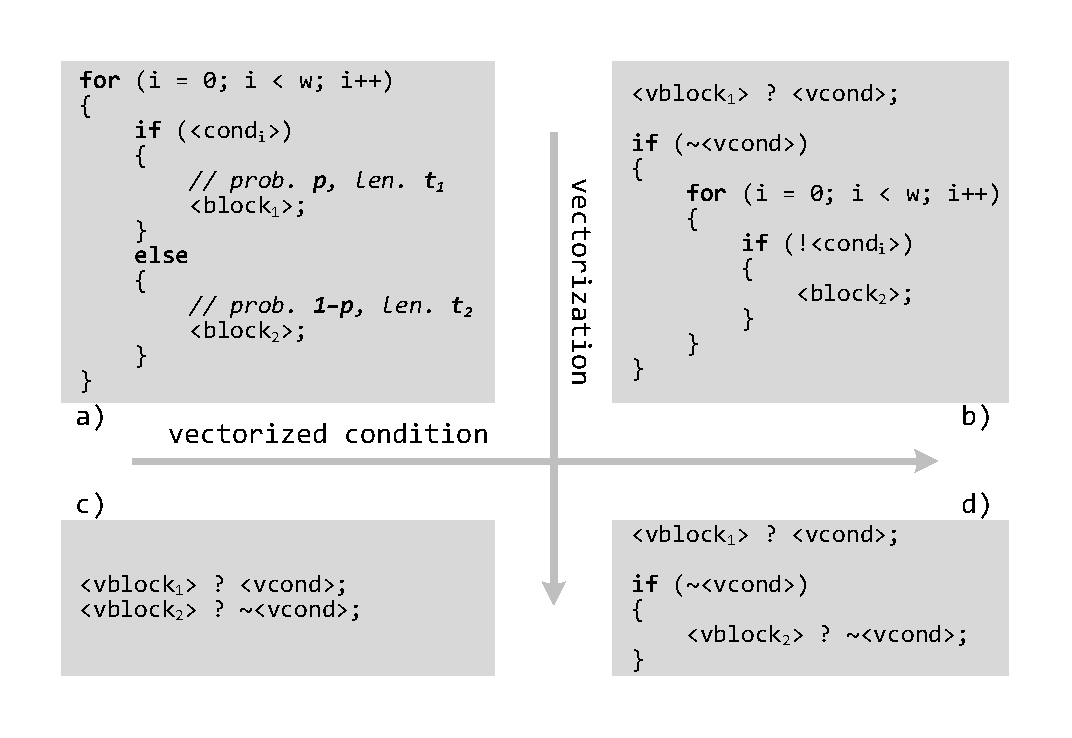
\includegraphics[width=0.65\textwidth]{pics/if_else_vectorization.pdf}
\captionstyle{normal}\caption{Please write your figure caption here.}\label{fig:1}
\end{figure}

The table contains data on the number of operations performed for the two considered examples of a flat cycle, in which the cycle body consists of one if-condition and one if-else-construction.

\begin{table}[!h]
\setcaptionmargin{0mm}
\onelinecaptionsfalse
\captionstyle{flushleft}
\caption{Operations count for \textbf{if} and \textbf{if-else} statements vectorization in flat loops.}
\bigskip
\begin{tabular}{|c|c|c|c|}
\hline
\textbf{if} statement & operations count & \textbf{if-else} statement & operations count \\
\hline
a) & $ptw$ & a) & $\left( pt_1 + (1 - p)t_2 \right)w$ \\
b) & $ptw$ & b) & $t_1 + (1 - p)t_2w$ \\
c) & $t$ & c) & $t_1 + t_2$ \\
d) & $\left( 1 - (1 - p)^w \right)t$ & d) & $t_1 + (1 - p^w)t_2$ \\
\hline
\end{tabular}
\end{table}

We will analyze only the second example from the if-else constructions (the first example is treated similarly). A fully vectorized cycle is more profitable than a cycle with a vectorized condition, if it contains fewer operations, that is, if the condition $t1 + t2 <= t1 + (1 - p) t2w$, or $(1 - p) w >= 1$ is satisfied. Thus, for the benefit of vectorization, either a high vectorization width, or a high probability of an alternative. If we consider the application of checking vectorized conditions for a fully vectorized cycle body, then we obtain the condition $t1 + (1 - p ^ w) t2 <= t1 + (1 - p) t2w$, which translates into $1 - p ^ w <= (1 - p) w$. This condition is disclosed in the following:

\begin{equation}
\sum_{i = 0}^{w - 1}{p^i} <= w
\end{equation}

This condition is obviously satisfied, since $p <= 1$, and the total terms are exactly w. Thus, we have obtained that using a fully vectorized loop body with a preliminary check of a vectorized condition for an unlikely branch is always more beneficial than using the original version of the code or condition vectoring. Note that this conclusion is true only under the assumption that the block1 linear segment is probable, and a vector code is always built for it.

We can consider the general case of vectorization of a flat cycle containing an arbitrary number of alternatives. Let the loop body contain n alternatives (with numbers from 0 to n - 1), each of which is executed with probability pi. In this case, we can neglect the operations of calculating conditions. It is also known that each alternative has a length ti. It is required to understand the conditions under which the use of vectorization is beneficial, as well as the application of checking vectorized conditions for a vector code. As in the previous examples, you can calculate the total number of running operations for a non-vectorized code; it is equal to the mathematical expectation of the number of operations per iteration of the loop multiplied by the number of iterations.

\begin{equation}
T = \left( \sum_{i = 0}^{n - 1}{p_it_i} \right) w
\end{equation}

With a complete cycle vectorization, the number of vector operations is of course equal to the sum of the lengths of all linear sections ti. Thus, the condition of the advantage of vectorization is the following equation:

\begin{equation}
\sum_{i = 0}^{n - 1}{t_i(p_iw - 1)} \ge 0
\end{equation}

In particular, it follows from this equation that if the loop body contains a large number of alternative execution branches with probabilities less than 1 / w, then vectoring of this loop cannot be beneficial. When adding checks of vectorized conditions for each of the cycle alternatives, we obtain the following equation for the advantage of vectorization.

\begin{equation}
\sum_{i = 0}^{n - 1}{t_i \left( p_iw - 1 + (1 - p_i) ^w \right) } \ge 0
\end{equation}

Consider this formula more closely. With a large number of alternatives, their probabilities are close to zero, so the term $(1 - pi) ^ w$ is a positive value not much less than one. From this we can conclude that the use of vectorized checks before performing vector versions of alternatives in the body of a flat cycle significantly increase the effect of vectorization. At least the theoretical estimates made in our assumptions indicate the benefits of applying such transformations. However, one should not forget that vector commands generally execute more slowly than their scalar counterparts. Moreover, the derivation of theoretical estimates did not take into account the influence of management operations and preparation of conditions, did not take into account the fact of the presence of possible dependencies between the calculation of conditions for various alternatives.

\section{Matrix operations vectorization}

In modern numerical methods used in high-performance computing, a special place is occupied by operations for working with vectors and matrices. In particular, one of the most critical operations is the multiplication of two matrices. Getting the product of two matrices, in which each row of the first matrix is multiplied by each column of the second matrix, is a heavy operation, which can take a significant part of the total program execution time. The presence of effective approaches to the implementation of this operation using the AVX-512 commands is necessary to increase the efficiency of the calculation codes using matrix calculations. In this section, we will consider the operations of multiplying small-size matrices (sizes 8 by 8, 7 by 7, 6 by 6 and 5 by 5) of the elements, which take, for example, up to 40\% of the work time of the domestic RANS / ILES calculation codes. In this case, the matrices under consideration are stored inside matrices of size 8 by 8 elements for reasons of alignment, as shown in Fig. N.

\begin{figure}[h]
\setcaptionmargin{5mm}
%\onelinecaptionsfalse % if the caption is multiline
\onelinecaptionstrue  % if the caption is one-line
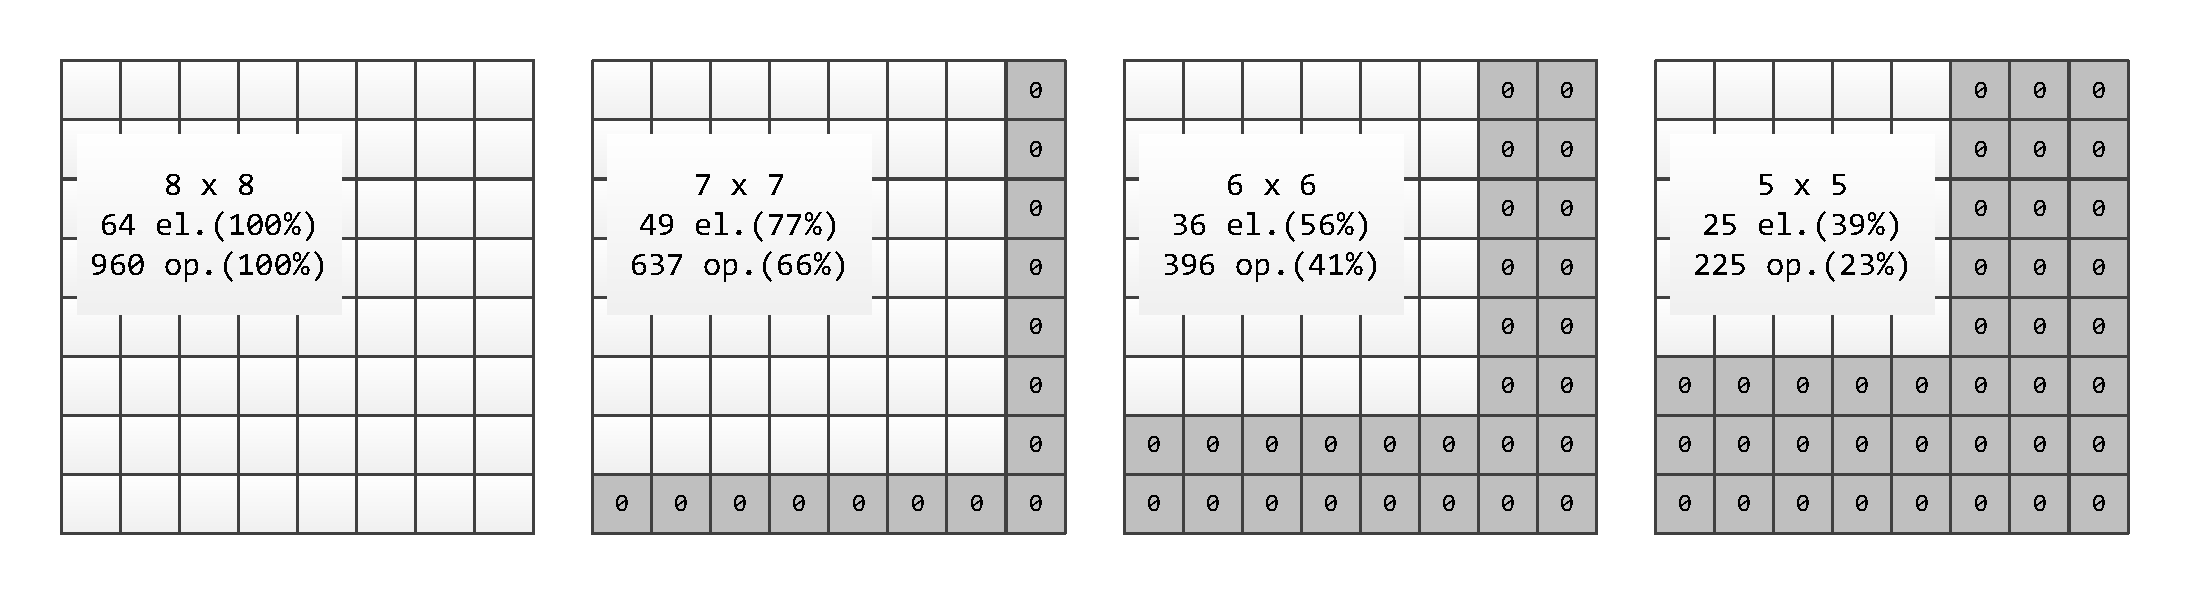
\includegraphics[width=0.85\textwidth]{pics/matrices_8x8_7x7_6x6_5x5.pdf}
\captionstyle{normal}\caption{Please write your figure caption here.}\label{fig:1}
\end{figure}

\begin{figure}[h]
\setcaptionmargin{5mm}
%\onelinecaptionsfalse % if the caption is multiline
\onelinecaptionstrue  % if the caption is one-line
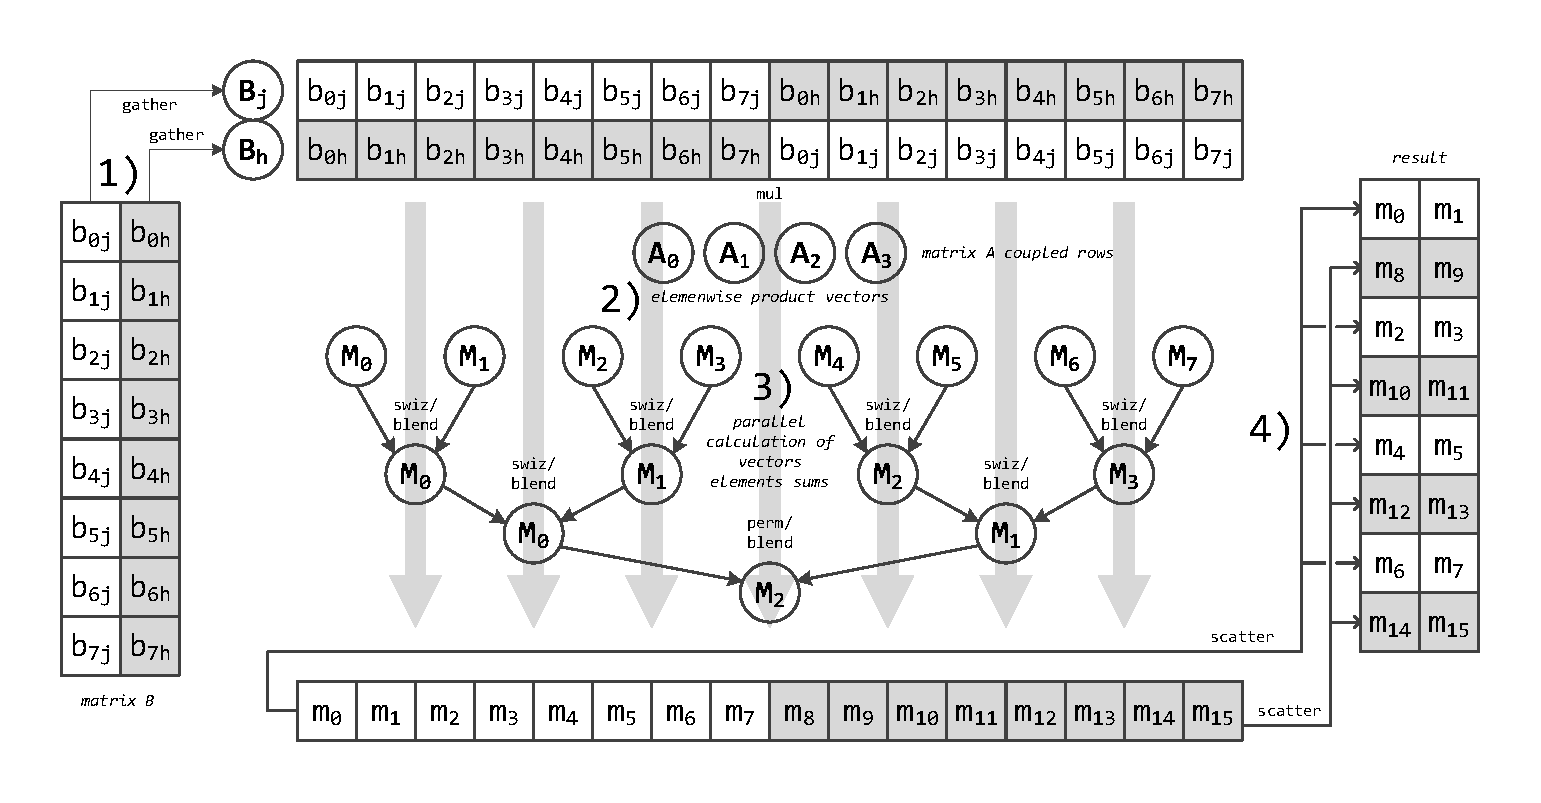
\includegraphics[width=0.85\textwidth]{pics/mmult_1.pdf}
\captionstyle{normal}\caption{Please write your figure caption here.}\label{fig:1}
\end{figure}

\begin{lstlisting}
#define SWIZ_2_ADD_2_BLEND_1(X, Y, SWIZ_TYPE, BLEND_MASK)         \
    _mm512_mask_blend_ps(BLEND_MASK,                              \
                         ADD(X, _mm512_swizzle_ps(X, SWIZ_TYPE)), \
                         ADD(Y, _mm512_swizzle_ps(Y, SWIZ_TYPE)))
#define PERM_2_ADD_2_BLEND_1(X, Y, PERM_TYPE, BLEND_MASK)              \
    _mm512_mask_blend_ps(BLEND_MASK,                                   \
                         ADD(X, _mm512_permute4f128_ps(X, PERM_TYPE)), \
                         ADD(Y, _mm512_permute4f128_ps(Y, PERM_TYPE)))

\end{lstlisting}

\begin{lstlisting}
void mul_8x8(float * __restrict a, float * __restrict b,
             float * __restrict r)
{
    ........................................
    __m512 bj, bj2,
           m0, m1, m2, m3, m4, m5, m6, m7;

    // Indices for matrix columns.
    __m512i ind_cc = _mm512_set_epi32(7*V8+1, 6*V8+1, 5*V8+1, 4*V8+1,
                                      3*V8+1, 2*V8+1,   V8+1,      1,
                                      7*V8  , 6*V8  , 5*V8  , 4*V8  ,
                                      3*V8  , 2*V8  ,   V8  ,      0);
    __m512i ind_st = _mm512_set_epi32(7*V8  , 7*V8+1, 5*V8  , 5*V8+1,
                                      3*V8  , 3*V8+1,   V8  ,   V8+1,
                                      6*V8+1, 6*V8  , 4*V8+1, 4*V8  ,
                                      2*V8+1, 2*V8  ,      1,      0);

    // Load the rows of matrix "a".
    __m512 a0 = LD(&a[0]);
    ........................................
    __m512 a3 = LD(&a[6 * V8]);

    // Matrix "b" columns loop.
    for (int j = 0; j < V8; j += 2)
    {
        bj = _mm512_i32gather_ps(ind_cc, &b[j], _MM_SCALE_4);
        bj2 = _mm512_permute4f128_ps(bj, _MM_PERM_BADC);

        // Matrix "a" rows on matrix "b" columns multiplication.
        m0 = MUL(a0, bj);
        m1 = MUL(a0, bj2);
        ........................................
        m6 = MUL(a3, bj);
        m7 = MUL(a3, bj2);

        // Parallel calculation of vectors sums of elements.
        m0 = SWIZ_2_ADD_2_BLEND_1(m0, m1, _MM_SWIZ_REG_CDAB, 0xAAAA);
        m1 = SWIZ_2_ADD_2_BLEND_1(m2, m3, _MM_SWIZ_REG_CDAB, 0xAAAA);
        m2 = SWIZ_2_ADD_2_BLEND_1(m4, m5, _MM_SWIZ_REG_CDAB, 0xAAAA);
        m3 = SWIZ_2_ADD_2_BLEND_1(m6, m7, _MM_SWIZ_REG_CDAB, 0xAAAA);
        m0 = SWIZ_2_ADD_2_BLEND_1(m0, m1, _MM_SWIZ_REG_BADC, 0xCCCC);
        m1 = SWIZ_2_ADD_2_BLEND_1(m2, m3, _MM_SWIZ_REG_BADC, 0xCCCC);
        m2 = PERM_2_ADD_2_BLEND_1(m0, m1, _MM_PERM_CDAB, 0xF0F0);

        // Store the result.
        _mm512_i32scatter_ps(&r[j], ind_st, m2, _MM_SCALE_4);
    }
\end{lstlisting}

\begin{equation}
\begin{cases}
r_{i0} = a_{i0}b_{00} + a_{i1}b_{10} + ... + a_{i7}b_{70} \\
... \\
r_{i7} = a_{i0}b_{07} + a_{i1}b_{17} + ... + a_{i7}b_{77} \\
\end{cases}
\end{equation}

\begin{equation}
\overline{r_i} = a_{i0}\overline{b_0} + a_{i1}\overline{b_1} + ... + a_{i7}\overline{b_7} \\
\end{equation}

\begin{equation}
\begin{cases}
r_{i+1,0} = a_{i+1,0}b_{00} + a_{i+1,1}b_{10} + ... + a_{i+1,7}b_{70} \\
... \\
r_{i+1,7} = a_{i+1,0}b_{07} + a_{i+1,1}b_{17} + ... + a_{i+1,7}b_{77} \\
\end{cases}
\end{equation}

\begin{equation}
\overline{r_{i+1}} = a_{i+1,0}\overline{b_0} + a_{i+1,1}\overline{b_1} + ... + a_{i+1,7}\overline{b_7} \\
\end{equation}

\begin{equation}
\left(\vcenter{\hbox{$\overline{r_i}$}\hbox{$\overline{r_{i+1}}$}}\right) =
\left(
\left(\vcenter{\hbox{$\overline{a_{i0}}$}\hbox{$\overline{a_{i+1,0}}$}}\right) \circ
\left(\vcenter{\hbox{$\overline{b_0}$}\hbox{$\overline{b_0}$}}\right)
\right) +
\left(
\left(\vcenter{\hbox{$\overline{a_{i1}}$}\hbox{$\overline{a_{i+1,1}}$}}\right) \circ
\left(\vcenter{\hbox{$\overline{b_1}$}\hbox{$\overline{b_1}$}}\right)
\right) +
\left(
\left(\vcenter{\hbox{$\overline{a_{i7}}$}\hbox{$\overline{a_{i+1,7}}$}}\right) \circ
\left(\vcenter{\hbox{$\overline{b_7}$}\hbox{$\overline{b_7}$}}\right)
\right)
\end{equation}

\begin{lstlisting}
void mul_8x8(float * __restrict a, float * __restrict b,
             float * __restrict r)
{
    ........................................
    // Vector duplication indices.
    __m512i ind_df = _mm512_set_epi32( 7,  6,  5,  4,  3,  2, 1, 0,
                                       7,  6,  5,  4,  3,  2, 1, 0);
    __m512i ind_ds = _mm512_set_epi32(15, 14, 13, 12, 11, 10, 9, 8,
                                      15, 14, 13, 12, 11, 10, 9, 8);

    // Load and duplicate all rows of the matrix "b".
    __m512 b0 = LD(&b[0]);
    __m512 b1 = _mm512_permutexvar_ps(ind_ds, b0);
    b0 = _mm512_permutexvar_ps(ind_df, b0);
    ........................................
    __m512 b6 = LD(&b[6 * V8]);
    __m512 b7 = _mm512_permutexvar_ps(ind_ds, b6);
    b6 = _mm512_permutexvar_ps(ind_df, b6);

    // Load all rows of the matrix "a".
    __m512 a0 = LD(&a[0]);
    ........................................
    __m512 a6 = LD(&a[6 * V8]);

    // 8 indices for select elements from matrix "a".
    __m512i ind_0 = _mm512_set_epi32( 8,  8,  8,  8,  8,  8,  8,  8,
                                      0,  0,  0,  0,  0,  0,  0,  0);
    ........................................
    __m512i ind_7 = _mm512_set_epi32(15, 15, 15, 15, 15, 15, 15, 15,
                                      7,  7,  7,  7,  7,  7,  7,  7);

// Main block of operations.
#define BLOCK(N, A)                           \
    ST(&r[N * V8],                            \
      FMADD(PERMXV(ind_0, A), b0,             \
        FMADD(PERMXV(ind_1, A), b1,           \
          FMADD(PERMXV(ind_2, A), b2,         \
            FMADD(PERMXV(ind_3, A), b3,       \
              FMADD(PERMXV(ind_4, A), b4,     \
                FMADD(PERMXV(ind_5, A), b5,   \
                  FMADD(PERMXV(ind_6, A), b6, \
                    MUL(PERMXV(ind_7, A), b7)))))))));

    // Calculate and store the result.
    BLOCK(0, a0);
    BLOCK(2, a2);
    BLOCK(4, a4);
    BLOCK(6, a6);

#undef BLOCK

}
\end{lstlisting}

\begin{table}[!h]
\setcaptionmargin{0mm}
\onelinecaptionsfalse
\captionstyle{flushleft}
\caption{Vectorization speedup for matrix 8x8, 7x7, 6x6, 5x5 operations.}
\bigskip
\begin{tabular}{|c|c|c|c|}
\hline
\textbf{Matrices Size} & \textbf{Old Vect} & \textbf{Full Unroll} & \textbf{New Vect} \\
\hline
8x8 & 2.69 & 3.69 & 5.86 \\
7x7 & 2.04 & 2.74 & 4.66 \\
6x6 & 1.38 & 2.29 & 3.68 \\
5x5 & 0.80 & 1.44 & 2.50 \\
\hline
\end{tabular}
\end{table}

\section{Vectorization of loops \protect\\
with irregular number of iterations}

\begin{lstlisting}
void shell_sort_k_i_w(float *m, int n, int k, int i, int w)
{
    int j = i;
    __mmask16 ini_mask = ((unsigned int)0xFFFF) >> (16 - w);
    __mmask16 mask = ini_mask;
    __m512i ind_j = _mm512_add_epi32(_mm512_set1+epi32(i),
                                     ind_straight);
    __m512 t, q;

    do
    {
        mask = mask & _mm512_mask_cmp_epi32_mask(mask, ind_j, ind_k,
                                                 __MM_CMPINT_GE);
        q = _mm512_mask_load_ps(q, mask, &m[j - k]);
        mask = mask & _mm512_mask_cmp_ps_mask(mask, t, q,
                                              __MM_CMPINT_LT);
        _mm512_mask_store_ps(&m[j], mask, q);
        ind_j = _mm512_mask_sub_epi32(ind_j, mask, ind_j, ind_k);
        j -= k;
    }
    while (mask != 0x0);
    
    _mm512_mask_i32scatter_ps(m, ini_mask, ind_j, t, _MM_SCALE_4);
}
\end{lstlisting}

\section{Physical calculations vectorization}

section

\section{Conclusion}

conclusion

\begin{acknowledgments}
We thank A.~A.~Surname1 and B.~B.~Surname2 for their participation in discussions of the results. We are grateful to C.~C.~Surname3 and the reviewers for careful reading of the manuscript and helpful remarks. Links to grants are also listed here.
\end{acknowledgments}

\begin{thebibliography}{99}

\bibitem{ex}
\refitem{article}
Doerfler D., Deslippe J., Williams S. et al., \textquotedblleft Applying the Roofline Performance Model to the Intel Xeon Phi Knights Landing Processor. ,\textquotedblright M. Taufer et al. (Eds.): ISC High Performance Workshops 2016, LNCS. - 2016. - vol. 9945. - pp. 339?353. DOI: 10.1007/978-3-319-46079-6.

\bibitem{ex}
\refitem{article}
Doerfler D., Deslippe J., Williams S. et al., \textquotedblleft Applying the Roofline Performance Model to the Intel Xeon Phi Knights Landing Processor. ,\textquotedblright M. Taufer et al. (Eds.): ISC High Performance Workshops 2016, LNCS. - 2016. - vol. 9945. - pp. 339?353. DOI: 10.1007/978-3-319-46079-6.

\bibitem{ex}
\refitem{article}
Doerfler D., Deslippe J., Williams S. et al., \textquotedblleft Applying the Roofline Performance Model to the Intel Xeon Phi Knights Landing Processor. ,\textquotedblright M. Taufer et al. (Eds.): ISC High Performance Workshops 2016, LNCS. - 2016. - vol. 9945. - pp. 339?353. DOI: 10.1007/978-3-319-46079-6.

\bibitem{ex}
\refitem{article}
Doerfler D., Deslippe J., Williams S. et al., \textquotedblleft Applying the Roofline Performance Model to the Intel Xeon Phi Knights Landing Processor. ,\textquotedblright M. Taufer et al. (Eds.): ISC High Performance Workshops 2016, LNCS. - 2016. - vol. 9945. - pp. 339?353. DOI: 10.1007/978-3-319-46079-6.

\bibitem{ex}
\refitem{article}
Doerfler D., Deslippe J., Williams S. et al., \textquotedblleft Applying the Roofline Performance Model to the Intel Xeon Phi Knights Landing Processor. ,\textquotedblright M. Taufer et al. (Eds.): ISC High Performance Workshops 2016, LNCS. - 2016. - vol. 9945. - pp. 339?353. DOI: 10.1007/978-3-319-46079-6.

\bibitem{ex}
\refitem{article}
Doerfler D., Deslippe J., Williams S. et al., \textquotedblleft Applying the Roofline Performance Model to the Intel Xeon Phi Knights Landing Processor. ,\textquotedblright M. Taufer et al. (Eds.): ISC High Performance Workshops 2016, LNCS. - 2016. - vol. 9945. - pp. 339?353. DOI: 10.1007/978-3-319-46079-6.

\bibitem{ex}
\refitem{article}
Doerfler D., Deslippe J., Williams S. et al., \textquotedblleft Applying the Roofline Performance Model to the Intel Xeon Phi Knights Landing Processor. ,\textquotedblright M. Taufer et al. (Eds.): ISC High Performance Workshops 2016, LNCS. - 2016. - vol. 9945. - pp. 339?353. DOI: 10.1007/978-3-319-46079-6.

\bibitem{ex}
\refitem{article}
Doerfler D., Deslippe J., Williams S. et al., \textquotedblleft Applying the Roofline Performance Model to the Intel Xeon Phi Knights Landing Processor. ,\textquotedblright M. Taufer et al. (Eds.): ISC High Performance Workshops 2016, LNCS. - 2016. - vol. 9945. - pp. 339?353. DOI: 10.1007/978-3-319-46079-6.

\bibitem{ex}
\refitem{article}
Doerfler D., Deslippe J., Williams S. et al., \textquotedblleft Applying the Roofline Performance Model to the Intel Xeon Phi Knights Landing Processor. ,\textquotedblright M. Taufer et al. (Eds.): ISC High Performance Workshops 2016, LNCS. - 2016. - vol. 9945. - pp. 339?353. DOI: 10.1007/978-3-319-46079-6.

\bibitem{ex}
\refitem{article}
Doerfler D., Deslippe J., Williams S. et al., \textquotedblleft Applying the Roofline Performance Model to the Intel Xeon Phi Knights Landing Processor. ,\textquotedblright M. Taufer et al. (Eds.): ISC High Performance Workshops 2016, LNCS. - 2016. - vol. 9945. - pp. 339?353. DOI: 10.1007/978-3-319-46079-6.

\bibitem{ex}
\refitem{article}
Doerfler D., Deslippe J., Williams S. et al., \textquotedblleft Applying the Roofline Performance Model to the Intel Xeon Phi Knights Landing Processor. ,\textquotedblright M. Taufer et al. (Eds.): ISC High Performance Workshops 2016, LNCS. - 2016. - vol. 9945. - pp. 339?353. DOI: 10.1007/978-3-319-46079-6.

\bibitem{ex}
\refitem{article}
Doerfler D., Deslippe J., Williams S. et al., \textquotedblleft Applying the Roofline Performance Model to the Intel Xeon Phi Knights Landing Processor. ,\textquotedblright M. Taufer et al. (Eds.): ISC High Performance Workshops 2016, LNCS. - 2016. - vol. 9945. - pp. 339?353. DOI: 10.1007/978-3-319-46079-6.

\bibitem{ex}
\refitem{article}
Doerfler D., Deslippe J., Williams S. et al., \textquotedblleft Applying the Roofline Performance Model to the Intel Xeon Phi Knights Landing Processor. ,\textquotedblright M. Taufer et al. (Eds.): ISC High Performance Workshops 2016, LNCS. - 2016. - vol. 9945. - pp. 339?353. DOI: 10.1007/978-3-319-46079-6.

\bibitem{ex}
\refitem{article}
Doerfler D., Deslippe J., Williams S. et al., \textquotedblleft Applying the Roofline Performance Model to the Intel Xeon Phi Knights Landing Processor. ,\textquotedblright M. Taufer et al. (Eds.): ISC High Performance Workshops 2016, LNCS. - 2016. - vol. 9945. - pp. 339?353. DOI: 10.1007/978-3-319-46079-6.

\bibitem{ex}
\refitem{article}
Doerfler D., Deslippe J., Williams S. et al., \textquotedblleft Applying the Roofline Performance Model to the Intel Xeon Phi Knights Landing Processor. ,\textquotedblright M. Taufer et al. (Eds.): ISC High Performance Workshops 2016, LNCS. - 2016. - vol. 9945. - pp. 339?353. DOI: 10.1007/978-3-319-46079-6.

\bibitem{ex}
\refitem{article}
Doerfler D., Deslippe J., Williams S. et al., \textquotedblleft Applying the Roofline Performance Model to the Intel Xeon Phi Knights Landing Processor. ,\textquotedblright M. Taufer et al. (Eds.): ISC High Performance Workshops 2016, LNCS. - 2016. - vol. 9945. - pp. 339?353. DOI: 10.1007/978-3-319-46079-6.

\bibitem{ex}
\refitem{article}
Doerfler D., Deslippe J., Williams S. et al., \textquotedblleft Applying the Roofline Performance Model to the Intel Xeon Phi Knights Landing Processor. ,\textquotedblright M. Taufer et al. (Eds.): ISC High Performance Workshops 2016, LNCS. - 2016. - vol. 9945. - pp. 339?353. DOI: 10.1007/978-3-319-46079-6.

\bibitem{ex}
\refitem{article}
Doerfler D., Deslippe J., Williams S. et al., \textquotedblleft Applying the Roofline Performance Model to the Intel Xeon Phi Knights Landing Processor. ,\textquotedblright M. Taufer et al. (Eds.): ISC High Performance Workshops 2016, LNCS. - 2016. - vol. 9945. - pp. 339?353. DOI: 10.1007/978-3-319-46079-6.

\bibitem{ex}
\refitem{article}
Doerfler D., Deslippe J., Williams S. et al., \textquotedblleft Applying the Roofline Performance Model to the Intel Xeon Phi Knights Landing Processor. ,\textquotedblright M. Taufer et al. (Eds.): ISC High Performance Workshops 2016, LNCS. - 2016. - vol. 9945. - pp. 339?353. DOI: 10.1007/978-3-319-46079-6.

\bibitem{ex}
\refitem{article}
Doerfler D., Deslippe J., Williams S. et al., \textquotedblleft Applying the Roofline Performance Model to the Intel Xeon Phi Knights Landing Processor. ,\textquotedblright M. Taufer et al. (Eds.): ISC High Performance Workshops 2016, LNCS. - 2016. - vol. 9945. - pp. 339?353. DOI: 10.1007/978-3-319-46079-6.

\bibitem{ex}
\refitem{article}
Doerfler D., Deslippe J., Williams S. et al., \textquotedblleft Applying the Roofline Performance Model to the Intel Xeon Phi Knights Landing Processor. ,\textquotedblright M. Taufer et al. (Eds.): ISC High Performance Workshops 2016, LNCS. - 2016. - vol. 9945. - pp. 339?353. DOI: 10.1007/978-3-319-46079-6.

\bibitem{ex}
\refitem{article}
Doerfler D., Deslippe J., Williams S. et al., \textquotedblleft Applying the Roofline Performance Model to the Intel Xeon Phi Knights Landing Processor. ,\textquotedblright M. Taufer et al. (Eds.): ISC High Performance Workshops 2016, LNCS. - 2016. - vol. 9945. - pp. 339?353. DOI: 10.1007/978-3-319-46079-6.

\bibitem{ex}
\refitem{article}
Doerfler D., Deslippe J., Williams S. et al., \textquotedblleft Applying the Roofline Performance Model to the Intel Xeon Phi Knights Landing Processor. ,\textquotedblright M. Taufer et al. (Eds.): ISC High Performance Workshops 2016, LNCS. - 2016. - vol. 9945. - pp. 339?353. DOI: 10.1007/978-3-319-46079-6.

\bibitem{ex}
\refitem{article}
Doerfler D., Deslippe J., Williams S. et al., \textquotedblleft Applying the Roofline Performance Model to the Intel Xeon Phi Knights Landing Processor. ,\textquotedblright M. Taufer et al. (Eds.): ISC High Performance Workshops 2016, LNCS. - 2016. - vol. 9945. - pp. 339?353. DOI: 10.1007/978-3-319-46079-6.

\bibitem{ex}
\refitem{article}
Doerfler D., Deslippe J., Williams S. et al., \textquotedblleft Applying the Roofline Performance Model to the Intel Xeon Phi Knights Landing Processor. ,\textquotedblright M. Taufer et al. (Eds.): ISC High Performance Workshops 2016, LNCS. - 2016. - vol. 9945. - pp. 339?353. DOI: 10.1007/978-3-319-46079-6.

\bibitem{ex}
\refitem{article}
Doerfler D., Deslippe J., Williams S. et al., \textquotedblleft Applying the Roofline Performance Model to the Intel Xeon Phi Knights Landing Processor. ,\textquotedblright M. Taufer et al. (Eds.): ISC High Performance Workshops 2016, LNCS. - 2016. - vol. 9945. - pp. 339?353. DOI: 10.1007/978-3-319-46079-6.

\bibitem{ex}
\refitem{article}
Doerfler D., Deslippe J., Williams S. et al., \textquotedblleft Applying the Roofline Performance Model to the Intel Xeon Phi Knights Landing Processor. ,\textquotedblright M. Taufer et al. (Eds.): ISC High Performance Workshops 2016, LNCS. - 2016. - vol. 9945. - pp. 339?353. DOI: 10.1007/978-3-319-46079-6.

\bibitem{ex}
\refitem{article}
Doerfler D., Deslippe J., Williams S. et al., \textquotedblleft Applying the Roofline Performance Model to the Intel Xeon Phi Knights Landing Processor. ,\textquotedblright M. Taufer et al. (Eds.): ISC High Performance Workshops 2016, LNCS. - 2016. - vol. 9945. - pp. 339?353. DOI: 10.1007/978-3-319-46079-6.

\bibitem{ex}
\refitem{article}
Doerfler D., Deslippe J., Williams S. et al., \textquotedblleft Applying the Roofline Performance Model to the Intel Xeon Phi Knights Landing Processor. ,\textquotedblright M. Taufer et al. (Eds.): ISC High Performance Workshops 2016, LNCS. - 2016. - vol. 9945. - pp. 339?353. DOI: 10.1007/978-3-319-46079-6.

\bibitem{ex}
\refitem{article}
Doerfler D., Deslippe J., Williams S. et al., \textquotedblleft Applying the Roofline Performance Model to the Intel Xeon Phi Knights Landing Processor. ,\textquotedblright M. Taufer et al. (Eds.): ISC High Performance Workshops 2016, LNCS. - 2016. - vol. 9945. - pp. 339?353. DOI: 10.1007/978-3-319-46079-6.

\end{thebibliography}

\end{document}
